\documentclass[12pt,t]{beamer}
\usepackage{graphicx}
\usepackage[vlined]{algorithm2e}
\usepackage{times}
\usepackage{calc}
\usepackage{url}
\usepackage{soul}
\usepackage{graphicx}
\usepackage{multirow, hhline}
\usepackage{array, booktabs}
\usepackage{amsmath}
\usepackage{amssymb}
\usepackage{relsize}
\usepackage{multirow}
\usepackage{booktabs}
\usepackage{pagecolor}
\usepackage{lipsum}
\usepackage{capt-of}
\usepackage{booktabs}

\usepackage{graphicx}
\usepackage{multicol}
\usepackage[T1]{fontenc}
\usepackage{ae}
\graphicspath{{fig/}}
\setbeameroption{hide notes}
\setbeamertemplate{note page}[plain]

\usetheme{default}
\beamertemplatenavigationsymbolsempty
\hypersetup{pdfpagemode=UseNone}

\usefonttheme{professionalfonts}
\usefonttheme{serif}
\usepackage{fontspec}
\setmainfont{Karla}
\setbeamerfont{note page}{family*=pplx,size=\footnotesize} % Palatino for notes

\definecolor{foreground}{RGB}{70,70,70}
\definecolor{background}{RGB}{249, 249, 249} %24,24,24
%\definecolor{title}{RGB}{107,174,214} %107,174,214
\definecolor{title}{RGB}{70,70,70}
\definecolor{gray}{RGB}{0,0,0}
\definecolor{subtitle}{RGB}{70,70,70}
\definecolor{hilight}{RGB}{102,255,204}
\definecolor{vhilight}{RGB}{255,111,207}

\setbeamercolor{titlelike}{fg=title}
\setbeamercolor{subtitle}{fg=subtitle}
\setbeamercolor{institute}{fg=gray}
\setbeamercolor{normal text}{fg=foreground,bg=background}


\setbeamercolor{item}{fg=foreground} % color of bullets
\setbeamercolor{subitem}{fg=gray}
\setbeamercolor{itemize/enumerate subbody}{fg=gray}
\setbeamertemplate{itemize subitem}{{\textendash}}
\setbeamerfont{itemize/enumerate subbody}{size=\footnotesize}
\setbeamerfont{itemize/enumerate subitem}{size=\footnotesize}

\setbeamercolor{block title}{fg=white,bg=gray!70}
\setbeamercolor{block body}{fg=black,bg=gray!10}
\setbeamercolor{block title alerted}{fg=red,bg=gray!40}
\setbeamercolor{block title example}{fg=black,bg=green!20}
\setbeamercolor{block body example}{fg=black,bg=green!5}
\setbeamerfont{block title}{series=\bfseries}

\hypersetup{colorlinks,linkcolor=foreground,urlcolor=foreground}


\setbeamertemplate{footline}{%
    \raisebox{5pt}{\makebox[\paperwidth]{\hfill\makebox[20pt]{\color{gray}
          \scriptsize\insertframenumber}}}\hspace*{5pt}}

\addtobeamertemplate{note page}{\setlength{\parskip}{12pt}}


\newcommand{\bi}{\begin{itemize}}
\newcommand{\ei}{\end{itemize}}
\newcommand{\ig}{\includegraphics}
\newcommand{\subt}[1]{{\footnotesize \color{subtitle} {#1}}}

\let\emph\relax % there's no \RedeclareTextFontCommand
\DeclareTextFontCommand{\emph}{\bfseries\em}


\setbeamertemplate{frametitle}
{\vskip4pt
  \leavevmode
%\hbox{%
\begin{beamercolorbox}[wd=\paperwidth,ht=2ex,dp=0ex]{frametitle}%
\underline{\makebox[\paperwidth][l]{\hspace*{10pt}
\large {{\insertframetitle}}}}
\end{beamercolorbox}
%  }%
}

%\setbeamercolor{frametitle}{fg=yellow,bg=red}

\begin{document}

\AtBeginSection[]{
  \begin{frame}
  \vfill
  \centering
  \begin{beamercolorbox}[sep=8pt,center,shadow=true,rounded=true]{title}
    \underline{\makebox[0.8\paperwidth][l]{
\large {{\insertsectionhead}}}}
  \end{beamercolorbox}
  \vfill
  \end{frame}
}

\title{\large{Lecture \#19: Support Vector Machines}}
\subtitle{CS 109A, STAT 121A, AC 209A: Data Science}
\author{Pavlos Protopapas \and Kevin Rader}
%\institute{Harvard University}
\date{}
\titlegraphic{
   
\includegraphics[height=2cm]{iacs}
\includegraphics[height=2cm]{hogwarts}
}
{
\setbeamertemplate{footline}{} % no page number here
\frame{
  \titlepage
  
}
}


\begin{frame}{Lecture Outline}
\tableofcontents
\end{frame}



%%%%%%%%%%%%%%%%%%%%%%%%%%%%%%%%%%%%%%%%%%%%%%%%%%%%%%%%%%%%%%%%%%%%%%%%%%%%%%
\section{Review}

%%%%%%%%%%%%%%
\begin{frame}{Classifiers and Decision Boundaries} 

Last time, we derived a linear classifier based on the intuition that a good classifier should
\vskip0.2cm
\begin{itemize}
\item maximize the distance between the points and the decision boundary (maximize margin)
\vskip0.2cm
\item misclassify as few points as possible
\end{itemize}
\end{frame}

%%%%%%%%%%%%%%
\begin{frame}{SVC as Optimization} 
\vskip-0.4cm
With the help of geometry, we translated our wish list into an optimization problem 
\[
\begin{cases}
\displaystyle \min_{\xi_n \in \mathbb{R}^{+}, w, b} \|w\|^2 + {\lambda\sum_{n=1}^N \xi_n}\\
\text{such that } y_n(w^\top x_n + b) \geq 1 - {\xi_n}, \; n = 1, \ldots, N
\end{cases}
\]
where $\xi_n$ quantifies the error at $x_n$. 
\vskip0.2cm
The SVC optimization problem is often solved in an alternate form (the dual form)
\[
\max_{\alpha_n\geq 0,\; \sum_{n} \alpha_ny_n = 0} \sum_{n} \alpha_n - \frac{1}{2} \sum_{n, m=1}^N y_ny_m\alpha_n\alpha_m x_n^\top x_m
\]
Later that this alternate form allows us to use SVC with non-linear boundaries.
\end{frame}

%%%%%%%%%%%%%%
\begin{frame}{Decision Boundaries and Support Vectors} 

\only<1>{
\vskip-0.4cm
If we remember how the error terms $\xi_n$'s were defined, we see that the points where $\xi_n = 0$ are precisely the support vectors
}
\only<2>{
\vskip-0.4cm
It's intuitive to see that to re-construct the decision boundary, \emph{only the support vectors are needed!}
}
\only<1-2>{
\begin{center}
\vskip0.2cm
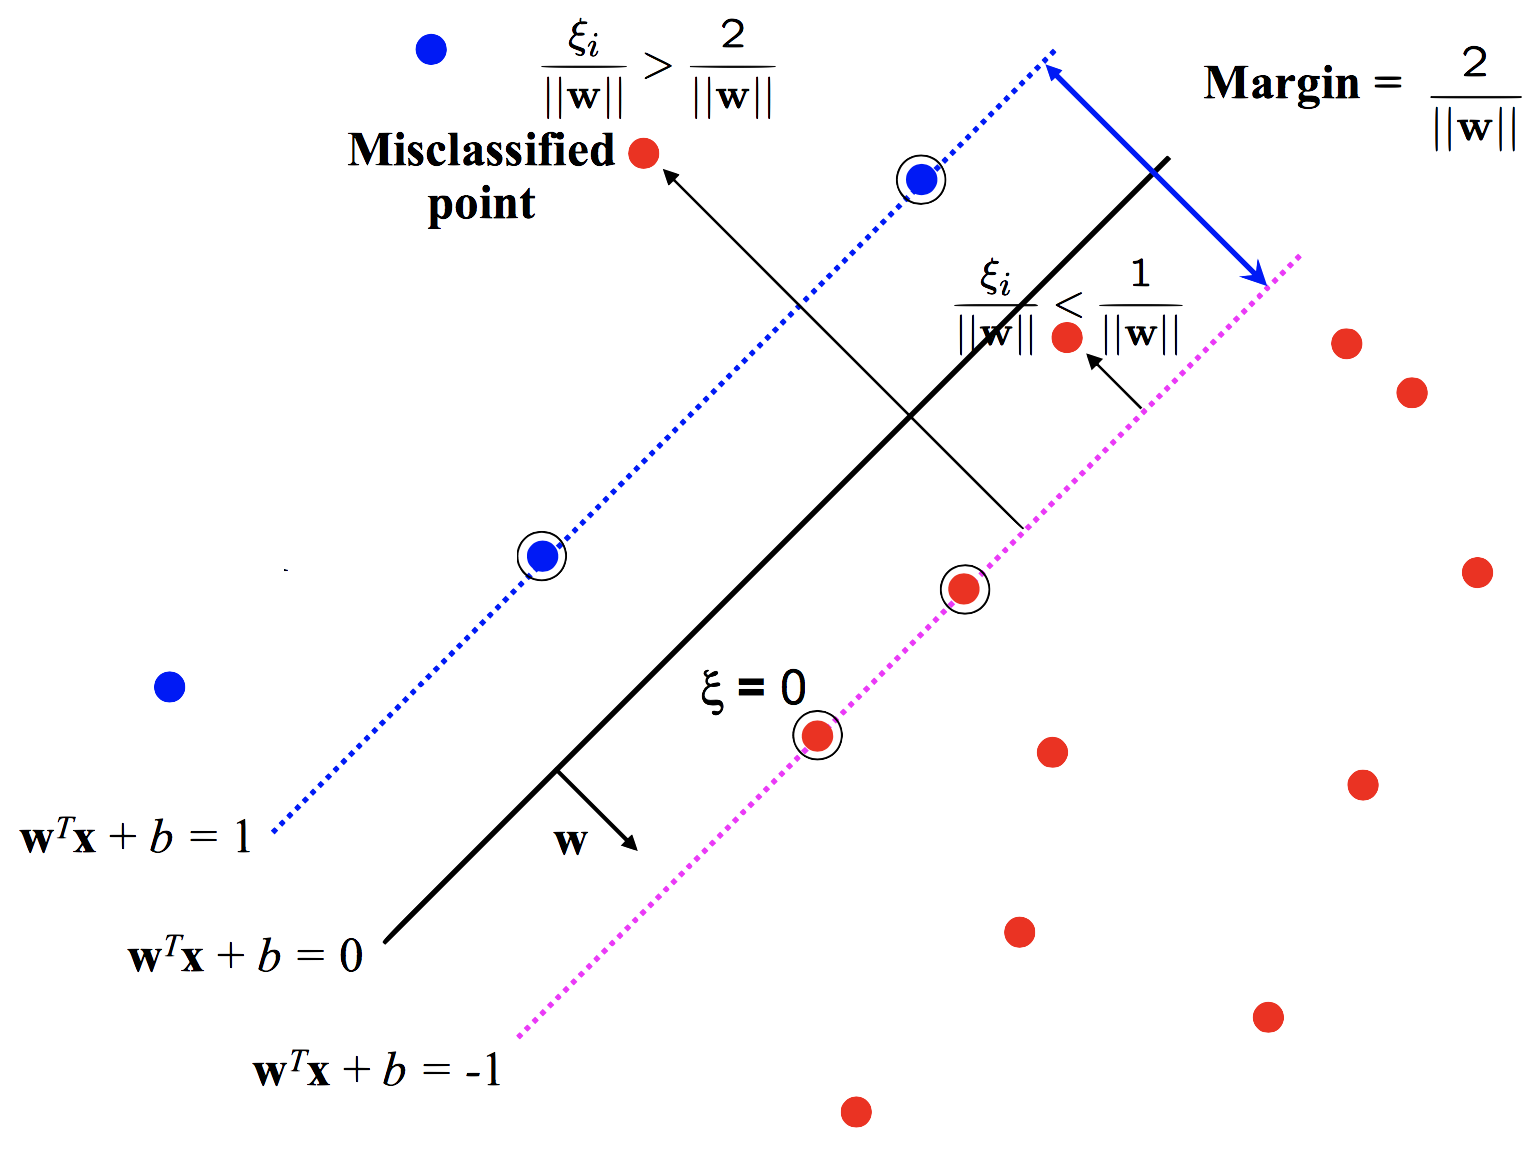
\includegraphics[width=75mm]{lecture18_g10}
\end{center}
}

\only<3>{
\begin{itemize}
\item The decision boundary of an SVC is given by
\[
\hat{w}^\top x + \hat{b} = \sum_{x_n\text{ is a support vector}} \hat{\alpha}_n y_n (x_n^\top x_n) + b
\]
where $\hat{\alpha}_n$ and the set of support vectors are found by solving the optimization problem.
\vskip0.2cm
\item To classify a test point $x_{test}$, we predict
\[
\hat{y}_{test} = \text{sign} \left(\hat{w}^\top x + \hat{b}\right)
\]
\end{itemize}
}
\end{frame}

%%%%%%%%%%%%%%%%%%%%%%%%%%%%%%%%%%%%%%%%%%%%%%%%%%%%%%%%%%%%%%%%%%%%%%%%%%%%%%
\section{Extension to Non-linear Boundaries}

%%%%%%%%%%%%%%
\begin{frame}{Polynomial Regression: Two Perspectives} 
\vskip-0.4cm
Given a training set 
\[
\{(x_1, y_1), \ldots, (x_N, y_N)\}
\]
with a single real-valued predictor, we can view fitting a 2nd degree polynomial model
\[
w_0  + w_1 x + w_2x^2
\]
on the data as the process of finding the best quadratic curve that fits the data. But in practice, we first expand the feature dimension of the training set
\[
x_n \mapsto (x^0_n, x^1_n, x^2_n)
\]
and train a \emph{linear model} on the expanded data
\[
\{(x^0_n, x^1_n, x^2_N, y_1), \ldots, (x^0_N, x^1_N, x^2_N, y_N)\}
\]
\end{frame}

%%%%%%%%%%%%%%
\begin{frame}{Transforming the Data} 
\vskip-0.4cm
The key observation is that training a polynomial model is just training a linear model on data with transformed predictors. 
\vskip0.2cm
In our previous example, transforming the data to fit a 2nd degree polynomial model requires a map
\begin{align*}
&\phi: \mathbb{R} \to \mathbb{R}^3\\
&\phi(x) = (x^0, x^1, x^2)
\end{align*}
where $\mathbb{R}$ called the \emph{input space}, $\mathbb{R}^3$ is called the \emph{feature space}. 
\vskip0.2cm
While the data is does not have a linear correlation in the input space $\mathbb{R}$, it may have one in the feature space $\mathbb{R}^3$.
\end{frame}

%%%%%%%%%%%%%%
\begin{frame}{SVC with Non-Linear Decision Boundaries} 

\only<1>{
\vskip-0.4cm
The same insight applies to classification: while the data may not be linear separable in the input space, it may be in a feature space after a fancy transformation:
\begin{center}
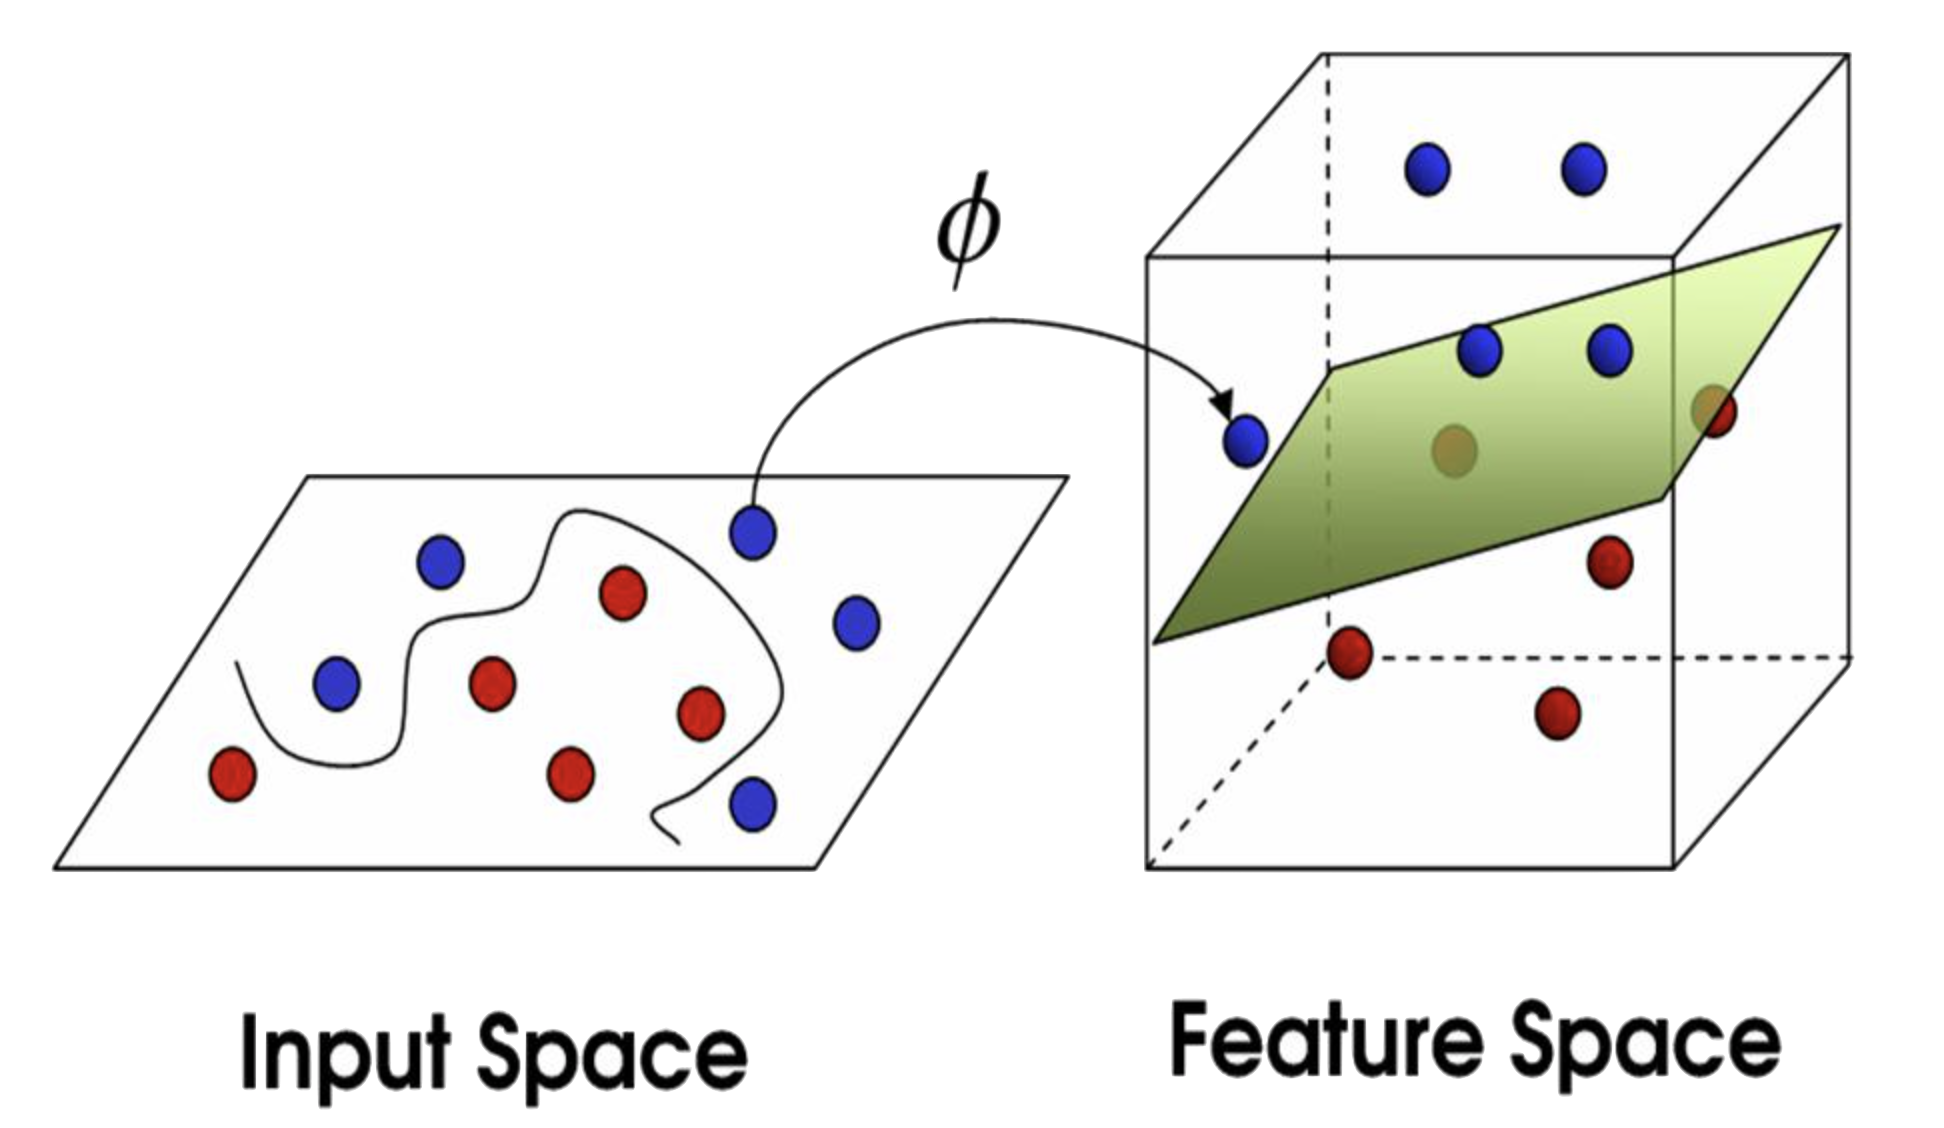
\includegraphics[width=90mm]{lecture19_g1}
\end{center}
}

\only<2>{
\textbf{The motto:} instead of tweaking the definition of SVC to accommodate non-linear decision boundaries. We map the data into a feature space in which the classes are linearly separable:
\vskip0.2cm
\begin{itemize}
\item Apply transform $\phi: \mathbb{R}^J \to \mathbb{R}^{J'}$ on training data
\[
x_n \mapsto \phi(x_n) 
\]
where typically $J'$ is much larger than $J$. 
\vskip0.2cm
\item Train an SVC on the transformed data
\[
\{ (\phi(x_1), y_1), \ldots, (\phi(x_N), y_N)\}
\]
\end{itemize}
}
\end{frame}



%%%%%%%%%%%%%%
\begin{frame}{The Kernel Trick} 
\only<1>{
Since the feature space $\mathbb{R}^{J'}$ is extremely high dimensional, computing $\phi$ explicitly can be costly. 
\vskip0.2cm
Instead, we note that computing $\phi$ is unnecessary. 
\vskip0.2cm
Recall that training an SVC involves solving the optimization problem
\[
\max_{\alpha_n\geq 0,\; \sum_{n} \alpha_ny_n = 0} \sum_{n} \alpha_n - \frac{1}{2} \sum_{n, m=1}^N y_ny_m\alpha_n\alpha_m \phi(x_n)^\top \phi(x_m)
\]
In the above, \emph{we are only interested in computing inner products $\phi(x_n)^\top \phi(x_m)$ in the feature space} and not the quantities $\phi(x_n)$. 
}

\only<2>{
\vskip-0.4cm
The \emph{inner product} between two vectors is a measure of the similarity of the two vectors.
\vskip0.2cm
\begin{block}{Definition}
Given a transformation $\phi: \mathbb{R}^J \to \mathbb{R}^{J'}$, from input space $\mathbb{R}^J$ to feature space $\mathbb{R}^{J'}$, the function $K: \mathbb{R}^J \times \mathbb{R}^J \to \mathbb{R}$ defined by
\[
K(x_n, x_m) = \phi(x_n)^\top \phi(x_m),\quad x_n, x_m \in  \mathbb{R}^J
\] 
is called the \emph{kernel function} of $\phi$. 
\vskip0.2cm
Generally, \emph{kernel function} may refer to any function $K: \mathbb{R}^J\times \mathbb{R}^J \to \mathbb{R}$ that measure the similarity of vectors in $\mathbb{R}^J$, without explicitly defining a transform $\phi$. 
\end{block}
}

\only<3>{
\vskip-0.4cm
For a choice of kernel $K$, 
\[
K(x_n, x_m) = \phi(x_n)^\top \phi(x_m)
\]
we train an SVC by solving 
\[
\max_{\alpha_n\geq 0,\; \sum_{n} \alpha_ny_n = 0} \sum_{n} \alpha_n - \frac{1}{2} \sum_{n, m=1}^N y_ny_m\alpha_n\alpha_m \alert{K(x_n, x_m)}
\]
Computing $K(x_n, x_m)$ can be done without computing the mappings $\phi(x_n), \phi(x_m)$. 
\vskip0.2cm
This way of training a SVC in feature space while without explicitly working with the mapping $\phi$ is called \emph{the kernel trick}.
}
\end{frame}

%%%%%%%%%%%%%%
\begin{frame}{Transforming Data: An Example} 
\vskip-0.4cm
\small
\begin{block}{Example}
Let's define $\phi: \mathbb{R}^2 \to \mathbb{R}^6$ by
\[
\phi\left([x_1, x_2]\right) = (1, \sqrt{2}x_1, \sqrt{2}x_2, x^2_1, x^2_2, \sqrt{2} x_1x_2)
\]
The inner product in the feature space is
\[
\phi\left([x_{11}, x_{12}]\right)^\top \phi\left([x_{21}, x_{22}]\right) = (1 + x_{11} x_{21} + x_{12} x_{22})^2
\]
Thus, we can directly define a kernel function $K: \mathbb{R}^2 \times \mathbb{R}^2  \to \mathbb{R}$ by
\[
K(x_1, x_2)  = (1 + x_{11} x_{21} + x_{12} x_{22})^2.
\]
Notice that we need not compute $\phi\left([x_{11}, x_{12}]\right)$, $\phi\left([x_{21}, x_{22}]\right)$ to compute $K(x_1, x_2)$.
\end{block}
\end{frame}

%%%%%%%%%%%%%%
\begin{frame}{Kernel Functions} 
\vskip-0.4cm
Common kernel functions include:
\vskip0.2cm
\begin{itemize}
\item \textbf{Polynomial Kernel}
\[
K(x_1, x_2) = (x_1^\top x_2 + 1)^d
\]
where $d$ is a hyperparameter
\vskip0.2cm
\item \textbf{Radial Basis Function Kernel}
\[
K(x_1, x_2) = \exp\left\{ -\frac{\| x_1 - x_2\|^2}{2\sigma^2} \right\}
\]
where $\sigma$ is a hyperparameter
\vskip0.2cm
\item \textbf{Sigmoid Kernel}
\[
K(x_1, x_2) = \tanh (\kappa x_1^\top x_2  + \theta)
\]
where $\kappa$ and $\theta$ are hyperparameters.
\end{itemize}
\end{frame}

%%%%%%%%%%%%%%%%%%%%%%%%%%%%%%%%%%%%%%%%%%%%%%%%%%%%%%%%%%%%%%%%%%%%%%%%%%%%%%
\section{A User's Guide to Support Vector Machines}

%%%%%%%%%%%%%%
\begin{frame}{Why Does SVM Work?} 
[Not filling these in until it's clear that this lecture is needed]
\end{frame}

%%%%%%%%%%%%%%
\begin{frame}{Choosing the Kernel Function} 
[Not filling these in until it's clear that this lecture is needed]
\end{frame}

%%%%%%%%%%%%%%
\begin{frame}{Strengths and Weaknesses of SVM} 
[Not filling these in until it's clear that this lecture is needed]
\end{frame}

\end{document}
